\documentclass[11pt]{article}

% PACKAGES
\usepackage{amsmath}
\usepackage{graphicx}
\usepackage{float}
\usepackage{lipsum}
\usepackage{multicol}
\usepackage{xcolor}
\usepackage{tabularx}
\usepackage{booktabs}
\usepackage{hyperref}
\usepackage{geometry}
\usepackage{enumitem}

% OPTIONS
\geometry{margin=2cm}
\hypersetup{
    colorlinks=true,
    linkcolor=darkgray,
    urlcolor=blue,
    citecolor=blue,
    pdfborder={0 0 0}
}
\setlist[itemize]{label=\scriptsize\textbullet}
\setlist[itemize]{noitemsep, topsep=1pt}
\setlist[enumerate]{noitemsep, topsep=1pt}

\begin{document}
    
    \begin{figure}[H]
        \raggedright
        
\includegraphics[scale=0.4]{images/polimi.png} \hfill 
\includegraphics[scale=0.3]{images/airlab.jpeg}
    \end{figure}
    
    \vspace{5mm}
    
    \begin{center}
        % Select between First and Second
        {\Large \textbf{ANNDL - First Homework Report}}\\
        \vspace{2mm}
        % Change with your Team Name
        {\Large \textbf{Neural Network November}}\\
        \vspace{2mm}
        % Team Members Information
        {\large Bettiati Matteo,}
        {\large Bianchi Lorenzo,}
        {\large Ostidich Francesco}\\
        \vspace{2mm}
        % Codabench Nicknames
        {betti,}
        {lolly,}
        {kello}\\
        \vspace{2mm}
        % Matriculation Numbers
        {258730,}
        {259946,}
        {259863}\\
        \vspace{5mm}
        \today
    \end{center}    
    \vspace{5mm}

\section{Introduction}

The challenge involves developing a neural network model for multiclass classification on a dataset of blood cell images.

Our initial approach was to inspect the dataset to understand the nature of the images we would be working with. 
During this process, we identified and removed several outlier images, to ensure the quality and consistency of data. 
We also noticed that the number of images per class was not equal, therefore we exploited augmentation in order to make the dataset classes balanced.

Given the relatively small size of the dataset given, we decided to initially approach the problem using transfer learning with a pre-trained model.
To balance computational efficiency and accuracy, we firstly selected small base models.
Eventually, we selected other models that were better suited to our purpose, incorporating fine-tuning to further enhance our performance.

\section{Operations on dataset}
The raw dataset consists of total of 13759 images designed for the classification of different types of blood cells. Each image is labeled with one of eight classes, representing various blood cell types: Basophil, Eosinophil, Erythroblast, Immature granulocytes, Lymphocyte, Monocyte, Neutrophil and Platelet.

Images size is 96x96, color space is RGB (3 channels), with \textit{uint8} data type.

\subsection{Exploratory Data Analysis}

The first step in a good machine learning pipeline is exploratory data analysis (EDA).
To perform EDA, we plotted a grid sorted by class, which allowed us to identify two types of outliers.
The first was a repeated image containing a watermark of Shrek that appeared across multiple classes. 
The second was a repeated image featuring a watermark of Rickroll in the Monocyte class.
Both outliers were easily removed, as they were identical images repeated without variations, making them straightforward to detect.
Those images are shown here below.

\begin{figure}[H]
    \centering
    \begin{minipage}{0.2\textwidth}
        \centering
        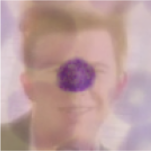
\includegraphics[width=\linewidth]{images/outlier1.png}
    \end{minipage}
    \hspace{2cm}
    \begin{minipage}{0.2\textwidth}
        \centering
        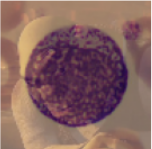
\includegraphics[width=\linewidth]{images/outlier2.png}
    \end{minipage}
\end{figure}

An analysis of class distribution revealed a mildly severe class imbalance. To address this issue, we employed image duplication and data augmentation to ensure more balanced representation across classes.

Additionally, we identified some ambiguously labeled images, such as the ones here below. Since there were no clearly mislabeled samples and considering the overall dataset size, we opted to retain these ambiguous images. This decision was made to preserve inherent diversity and sparsity in the dataset, which can contribute to the robustness of the model.

\begin{figure}[H]
    \centering
    \begin{minipage}{0.2\textwidth}
        \centering
        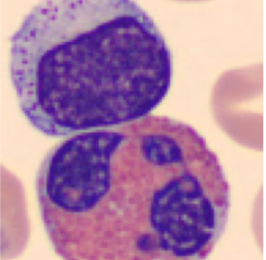
\includegraphics[width=\linewidth]{images/ambiguous1.png}
    \end{minipage}
    \hspace{2cm}
    \begin{minipage}{0.2\textwidth}
        \centering
        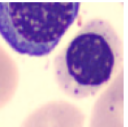
\includegraphics[width=\linewidth]{images/ambiguous2.png}
    \end{minipage}
\end{figure}

\subsection{Data augmentation}

Data augmentation has been a paramount stage which influenced greatly the performance of the model.
The progressive refinement of the pipeline lead to 3 main iterations of data augmentation pipeline.
All of which handled class unbalance and performed data splitting either by custom functions or using \textit{train\_test\_split} by \textit{scikit\-learn}.

In the first place, 150 images per class were reserved for a test set.
Those images were themselves augmented, in order to provide higher generality precision when evaluating the trained models.

\subsubsection{Initial augmentation}

The first round of augmentation was relatively simple compared to the subsequent iterations.
It included the following functions, each applied with random intensity:

\begin{itemize}
    \item random flip;
    \item random rotation;
    \item random brightness;
    \item random contrast;
    \item random stretch;
    \item random hue;
    \item random blur;
    \item random saturation.
\end{itemize}

Both original and augmented images were included in this dataset. 
However, care was taken to ensure that different versions of the same image were not included in both the training and validation sets.
Each image was augmented multiple times to reach the quota of 2,500 elements per class.

\subsubsection{Static augmentation}

The second round utilized additional functions to achieve a higher level of augmentation. 
The following functions were used:

\begin{itemize}
    \item random blur;
    \item random flip;
    \item random rotation;
    \item random brightness;
    \item random hue;
    \item random contrast;
    \item random grid mask;
    \item random color degeneration;
    \item random cutout;
    \item random saturation;
    \item random shear.
\end{itemize}

A random selection of a random size of functions, each with a random intensity, was applied on each augmented image.
Original images were excluded from the dataset at this stage. 
Each image was augmented as many times as to reach 3,000 elements per class.

For the final submissions, the best models trained on this dataset were retrained using a dataset with the same augmentation level, now including all test set images. 
Additionally, the number of elements per class was increased to 5,000.

\subsubsection{Dynamic augmentation}

The third approach, which was ultimately used in the final submission model, began by balancing the label distribution.
This was achieved by duplicating the underrepresented classes just enough to match the number of samples in the largest class.
The entire dataset was then split and fed into a \textit{TensorFlow Dataset}, which managed the batch size, shuffling, and mapping of the augmentation pipeline.
% FIXME lolly che vor di "TensorFlow Datasets"

This approach made the augmentation process dynamic rather than static, as augmentations were applied in real-time during runtime. 
By handling augmentations dynamically, the model was exposed to a broader variety of augmented samples, enhancing generalization and reducing the risk of overfitting.
However, this method was adopted only as a last resort, as it significantly slowed down the training process, even though it was a necessary step to achieve the final performance.

\subsection{Preprocessing data}

All the pre-trained models we selected came with an already implemented data preprocessing phase.

Initially, before using augmentation to balance the classes of the dataset, we opted for utilizing the \textit{class\_weight} function to adjust the weights, since the dataset was unbalanced.
However, after performing data augmentation to balance the classes, we no longer needed to use this function.

\section{Model experiments}

Each team member began by selecting a pre-trained model, and while tweaking hyperparameters and top layers structure, we started to look for the best resulting ones to use.

We started with relatively small models, like \textit{MobileNetV2}, a model known for its favorable trade-off between parameter count and accuracy, as the foundation for our experiments, to leverage fast training and less overfitting risk given the small dataset.

Following this initial setup, we proceeded to design the top layers architecture. 
Overall, while the specific structures varied slightly between attempts, the core design remained consistent.

\begin{table}[h!]
    \centering
    \begin{tabular}{|c|}
        \hline
        \textbf{Layer type} \\ \hline
        Input layer \\ \hline
        Pre-trained base model \\ \hline
        Global average pooling 2D \\ \hline
        Dense \\ \hline
        Batch normalization \\ \hline
        Dropout \\ \hline
        Dense \\ \hline
        Batch normalization \\ \hline
        Dropout \\ \hline
        Output layer \\ \hline
    \end{tabular}
\end{table}

Hyperparameter have been also changing a lot during the development phase; here we are just going to show the most used ones.
In the hyperparameter tuning section you can find all the values that have been used and how they affected our models.
Here after a recap with the most used ones.

\begin{table}[h!]
    \centering
    \begin{tabular}{|c|c|c|}
        \hline
        \textbf{Parameter} & \textbf{Pre-training} & \textbf{Fine tuning} \\ \hline
        Learning rate & 1e-4 & 1e-5 \\ \hline
        Weight decay & 1e-3 & 1e-3 \\ \hline
        Epochs & 10 & 20 \\ \hline
        Batch size & 64 & 128 \\ \hline
    \end{tabular}
\end{table}

\subsection{Transfer learning}

From the start, we planned to divide the transfer learning training process in two phases: an initial phase focused on the top layers, followed by a fine-tuning phase mane on the base model, once accuracy plateaued.
This strategy aimed to enable the model to better leverage the pre-trained weights. 
To mitigate overfitting, we implemented early stopping, learning rate schedulers, dropout, and regularization techniques.

All the training was conducted using Colab and Kaggle GPUs.
To address resource limitations, we exploited checkpoints and mixed precision while training. Additionally, in some runs, \textit{TensorFlow Datasets} were employed to optimize RAM usage during training.
% FIXME lolly che vor di "TensorFlow Datasets"

\subsection{Fine tuning}

After achieving a plateau in performance during the top layer training phase, we transitioned to fine tuning. 
This process involved unfreezing layers of the base model, allowing it to adjust weights to better fit the specific patterns in our dataset. 
Fine-tuning permitted more targeted adjustments, leveraging the general features recognition that had been learned during the top layer pre-training phase, while adapting to the nuances of our data.

Initially, we used to unfroze all layers at once. 
However, we later adopted a more gradual and widely recommended approach, unfreezing layers incrementally. 
Gradual unfreezing helps preventing the pre-trained model from completely overwriting its previously learned representations, preserving useful features while allowing adaptation. Unfreezing all layers at once can lead to catastrophic forgettings, where the model looses valuable general knowledge obtained from pre-training.
This gradual approach also reduces the risk of overfitting, as early layers (which often capture fundamental features like edges and textures) remain relatively stable during the initial stages of fine tuning.

\section{Comparison overview}

The first model used were tested and trained on the first augmented datasets.
Later on we switched to new augmented datasets. Some models were anyway been discard already. 
For this reason, some values may be misleading.

\subsection{Base model evaluation}

Initially, we selected a set of pre-trained models to evaluate as foundation for our end-goal model.
Below, we summarize the key metrics observed during this evaluation phase, which ultimately led us to focus on the \textit{MobileNetV2}, \textit{EfficientNetV2M} and \textit{ConvNeXtSmall} models.

\begin{table}[h!]
    \centering
    \begin{tabular}{|c|c|c|c|}
        \hline
        \textbf{Model Name} & \textbf{Pre-training} & \textbf{Fine tuning} & \textbf{Local accuracy} \\ \hline
        Xception            &  &  & \\ \hline
        ResNet152V2         & 0.70 & 0.92 & \\ \hline
        InceptionV3         &  & 0.90 & \\ \hline
        InceptionResNetV2   &  &  & \\ \hline
        MobileNetV2         & 0.5102 & 0.9163 & 0.9151 \\ \hline
        DenseNet201         & 0.78 & 0.91 & \\ \hline
        EfficientNetB4      & 0.7084 & 0.8436 & 0.8809 \\ \hline
        EfficientNetV2S     & 0.6898 & 0.8844 & 0.9321 \\ \hline
        EfficientNetV2M     &  &  & \\ \hline
        ConvNeXtTiny        &  &  & \\ \hline
        ConvNeXtSmall       &  &  & \\ \hline
    \end{tabular}
\end{table}

\subsection{Hyperparameter tuning}

% TODO spacca tutto kello

\section{Final model}

% TODO spacca tutto lolly

\section{Contributions}

All the members of the team contributed equally to the project. 
Here is a list of the main work tasks to which that each member contributed the most.

\begin{itemize}
    \item Bettiati helped with the setup of the work environment, training and testing new models, and fine tuning the parameters in order to find the best performing ones.
    \item Bianchi worked on data, by cleaning the dataset and providing the final dynamic augmentation used for the final model, while helping with the models training.
    \item Ostidich worked on the initial data augmentation, for then focussing on the hyperparameter tuning and testing process.
\end{itemize}

\section{References}

\begin{itemize}
    \item Artificial Neural Networks and Deep Learning (Polimi, AY 2024/2025): course slides.
\end{itemize}

\end{document}
